\chapter{LITERATURE REVIEW}
The issue of mobile robot navigation is something that a lot of people in schools are looking at. People are still trying to figure out how to make it better. They are working on things like figuring out where the robot is seeing what is around it planning a path and making it move. This part of the book looks really closely at the ideas and technologies that make indoor parcel-delivery systems work.New navigation systems are really good at making maps of the area and finding things that're in the way. They can also plan a path that's safe and works well. These systems use platforms like ROS 2 that help all the parts talk to each other.Also because of advances, in computer vision, deep learning and simulated environments autonomous robots are becoming more reliable and easier to use. Autonomous mobile robot navigation is getting better because of these things. Autonomous mobile robot navigation systems are being used in places now.
\section{Background}


The ideas talked about in this paper are the plan for the idea and actual creation of autonomous indoor delivery robots. To design systems we need to really understand how navigation works, how to figure out where the robot is, how to plan its path how to control its movement and how to put all the parts together. The following ideas are what tell us how to make the autonomous delivery robot work, in the world they help us decide which algorithms, sensor packages and software architectures to use to make autonomous indoor delivery robots work well.

Mobile robot navigation fundamentally depends on understanding the kinematic constraints of the robot platform. Differential drive robots, such as the TurtleBot3, operate under nonholonomic kinematic constraints, meaning they cannot move freely in all directions at a single instant. Instead, their motion is restricted to movements that are physically achievable through wheel rotations.

In differential-drive robots, we essentially drive the movements of two wheels on (one on each side of) the chassis that are driven independently by two motors. That is because the coordinated actuation of said wheels determines the linear velocity of the robot v and the angular velocity of the robot, which is 0. These input commands have a direct impact on the pose of the robot, its position and orientation in a global frame. The kinematic correlation between the inputs of the velocity and the change of pose is given as:

\begin{equation}
\begin{bmatrix}
\dot{x} \\
\dot{y} \\
\dot{\theta}
\end{bmatrix}
=
\begin{bmatrix}
v \cos(\theta) \\
v \sin(\theta) \\
\omega
\end{bmatrix}
\end{equation}

where:
\begin{itemize}[noitemsep]
\item $x, y$ represent the robot's position in the global coordinate frame
\item $\theta$ represents the robot's heading angle (orientation)
\item $\dot{x}, \dot{y}$ represent linear velocity components along the x and y axes
\item $v$ represents linear velocity
\item $\omega$ represents angular velocity
\end{itemize}

These kinematic constraints limit the robot's ability to execute arbitrary motion trajectories. Consequently, real world navigation needs to smooth path, plan trajectory and offer proper motion control measures to have viable and steady movement of a robot.

\subsection{Autonomous Mobile Robot Navigation Fundamentals}



The idea of autonomous mobile robot navigation is to allow robots to navigate in a safe and efficient way in a given environment. There are generally localization, mapping, path planning, obstacle avoidance, and motion control aspects of the navigation systems. These modules enable robots to know their locations, learn about the surrounding structures, design collision-free fields of movement and implement movement directions. Indoor delivery robotic systems are built on the incorporation of these elements of navigation within warehouses, hospitals, and academic institutions.
\subsection{Trajectory Smoothing and Interpolation}

Raw paths from planning algorithms like grid-based or sampling-based planners often have turns.These paths also have curvature and are not feasible for robots with kinematic constraints.The sharp turns and discontinuous curvature cause difficulties for differential drive robots.These robots need to follow motion profiles and meet their nonholonomic constraints.Differential drive robots have trouble, with paths that have turns.Their motion profiles must be smooth and continuous.They also have to comply with their constraints.. To overcome these constraints, they use trajectory smoothing to turn discrete paths represented as waypoints into continuous and differentiable paths with the use of waypoints as prongs of a path representation ~\cite{ravankar2018path}. This process is based on the technique of interpolation methods to produce smooth curves that must satisfy the velocity conditions, deceleration conditions and curvature conditions necessary to obtain stable robotic movement. When the sudden directional changes due to the trajectory smoothing are removed, the tracking accuracy would be improved, the mechanical forces acting on the actuators would be reduced, and the efficiency of the whole-navigation system would be raised.  

These methods that use spline interpolations are very useful for smoothing trajectories, as are interpolation methods. This is because spline interpolations are very flexible and are mathematically meaningful. There are a types of spline interpolations but the most common ones are cubic splines and B-splines.Cubic splines are good because they make curves that're smooth and have no sharp turns. They ensure that the position, velocity and acceleration of each section of the curve are the same. This means that cubic splines can follow the set of waypoints for which we are given and the transitions between them are smooth.The cubic splines and B-splines are important, for interpolation methods based on spline interpolations. B-splines have the opposite characteristics, however, because they are not strictly interpolated but only approximated the waypoints. The nature of this gives B-splines the ability to generate more smooth trajectories with finite curvature which is particularly useful in mobile robot motion tracking when using motion tracking controllers. The generated trajectory is dynamically realistic and can be synthesised by control algorithms, and can be used by differential-drive robots to follow predetermined trajectories safely and efficiently, due to the use of spline-based smoothing to ensure the trajectory is dynamically realistic.

\textbf{Natural Cubic Spline Interpolation for Path Smoothing}

Mobile robots require a smoothing algorithm for navigation, since many algorithms like A* and RRT produce piecewise-linear paths with abrupt changes in direction. Such non-circular motions are in contradiction to the kinematic constraints of differential-drive robots, which leads to jerky motions, loss of tracking accuracy and mechanical fatigue. The discrete sequence of waypoints is converted to a continuous curve by trajectory smoothing methods, that are kinematically allowed, yet are continuous and differentiable, and could be actually executed by a robot by using continuously differentiable curves.

The natural cubic splines are very popular as an interpolation method in robotics, due to their smoothness and ease of computation, as well as the fact that they are naturally easy to interpolate. A natural cubic spline is a discontinuous cubic polynomial that passes through each one of the given waypoints and is continuous at both the first and second derivatives at all of the continuity points.

These derivative conditions ensure that the resulting trajectory has smooth velocity and acceleration profiles which are essential in the realization of stable and compliant motion control.
\textbf{Mathematical Definition of Natural Cubic Splines}
The mathematical expression of natural cubic splines is in line with standard numerical 
analysis approaches~\cite{siciliano2016springer}.
Given a sequence of n + 1 waypoints $(x_0, y_0), (x_1, y_1), \ldots, (x_n, y_n)$, a natural cubic spline $S(t)$ consists of n cubic polynomial segments:

\begin{equation}
S_i(t) = a_i + b_i(t - t_i) + c_i(t - t_i)^2 + d_i(t - t_i)^3, \quad t \in [t_i, t_{i+1}]
\end{equation}

where $i = 0, 1, \ldots, n - 1$, and $t$ is a parameter (typically arc length or normalized distance).

The spline coefficients $(a_i, b_i, c_i, d_i)$ are determined by enforcing the following constraints:

\begin{enumerate}[noitemsep]
\item \textbf{Interpolation:} The spline passes through all waypoints:
\begin{align}
S_i(t_i) &= y_i \quad \text{and} \quad S_i(t_{i+1}) = y_{i+1}
\end{align}

The spline coefficients $(a_i, b_i, c_i, d_i)$ are obtained by satisfying the following conditions:
\begin{equation}
S_i'(t_{i+1}) = S_{i+1}'(t_{i+1}), \quad i = 0, 1, \ldots, n - 2
\end{equation}

\item \textbf{$C^2$ Continuity:} Second derivatives at the end points are zero:
\begin{equation}
S_i''(t_{i+1}) = S_{i+1}''(t_{i+1}), \quad i = 0, 1, \ldots, n - 2
\end{equation}

\item \textbf{Natural Boundary Conditions:} Second derivatives at the endpoints are zero:
\begin{equation}
S_0''(t_0) = 0 \quad \text{and} \quad S_{n-1}''(t_n) = 0
\end{equation}
\end{enumerate}

These restrictions give rise to a tridiagonal matrix system of $(n+1)$ linear equations, which can be solved efficiently via tridiagonal matrix methods. The natural boundary condition guarantees that the curve that is obtained is the ``smoothest'' possible interpolation that minimizes the total curvature energy.

\textbf{Parametric Representation for Robot Path Planning}
The standard $y = f(x)$ form is not used for mobile robot trajectories in 2D space; instead, a parameterization is used. Both x and y coordinates are functions of a parameter $t$ in parametric form:

\begin{equation}
P(t) = \begin{bmatrix} x(t) \\ y(t) \end{bmatrix}
\end{equation}

where \(x(t)\) and \(y(t)\) represent natural cubic splines that are independently fitted to the \(x\)- and \(y\)-coordinates of the waypoints, respectively.

\textbf{Why Parametric Representation?}

\begin{itemize}[noitemsep]
\item \textbf{Handles Vertical Segments:} Unlike standard splines, which require monotonically increasing \(x\)-values and therefore cannot accurately represent vertical or looping paths, parametric splines eliminate this limitation by treating both coordinates as functions of a common parameter.
\end{itemize}

\subsection{Localization and Mapping Principles}

Accurate localization and environmental mapping are essential for reliable robot navigation.Simultaneous localization and mapping, also known as SLAM, represent an important category of methods that enables robotic systems to build detailed maps of the previously unknown space and also determine their own location on the map. These types of SLAM utilize large collections of sensors to collect high-fidelity environmental data such as visual cameras, laser scanning systems (LiDAR) and inertial measurement systems (IMU). Combining these sensory signals, the mappings do not only enable the detection of obstacles and the recognition of landmarks in the navigation process, but also provide the basis of designing strong and effective path-planning algorithms.
\subsection{Path Planning and Obstacle Avoidance Fundamentals}

	Path planning focuses on generating optimal and collision-free trajectories between start and destination points.Simultaneous localization and mapping, also known as SLAM, represent an important category of methods that enables robotic systems to build detailed maps of the previously unknown space and also determine their own location on the map. These types of SLAM utilize large collections of sensors to collect high-fidelity environmental data such as visual cameras, laser scanning systems (LiDAR) and inertial measurement systems (IMU). Combining these sensory signals, the mappings do not only enable the detection of obstacles and the recognition of landmarks in the navigation process, but also provide the basis of designing strong and effective path-planning algorithms.

\subsection{Motion Control and Trajectory Tracking}

Motion control strategies help robots follow planned paths and move smoothly. They do this while staying stable.Traditional control methods, like Proportional-Integral-Derivative regulators are widely used to control the speed of motors and follow set paths.Advanced methods, Model Predictive Control work better for navigation. Model Predictive Control does this because it can predict what the robot will do in the future and control its movements to work best with the situation and any limitations of the robot and its environment.Model Predictive Control is a type of motion control strategy that helps robots navigate.
\subsection{Robotics Middleware and System Integration}

\begin{sloppypar}
	Robotic middleware platforms provide communication and integration frameworks that connect perception, navigation, and control modules. As it has been mentioned, the Robot Operating System 2.0 offers a modular architecture, the real-time facilitation of communication, and scalability, thus supporting autonomous robotic platforms. ROS2 enables the easy addition of perception algorithms, navigation stacks, simulation systems and user-interface systems, thus facilitating the development of complex autonomous delivery systems.
\end{sloppypar}

\section{Related Technologies}

Path planning is one of the problems in autonomous mobile robotics. Find a route from a start location to a target location without hitting anything in the way. This walk should be efficient as well. The path planner is extremely crucial as it impacts on the safety of the navigation, the smoothness of all the processes and the efficiency of time. Lots of algorithms have been proposed. Each one has its good and bad points like how good the path is, how much it costs to compute and how well it works in environments that are changing.In this section we will look at new path planning algorithms. We will also go though the reason for selecting the Improved A* algorithm for this project.

\subsection{Related Technology 1 -- Path Planning Algorithms}
Path planning is an issue in autonomous mobile robotics. We need to find a path, from a start location to a target without hitting anything. This path also needs to be efficient. The path planner is really important because it affects how safe the navigation is, how smooth everything runs and how well it works in time. There are a lot of algorithms that people have suggested. Each one has its good and bad points like how good the path is, how much it costs to compute and how well it works in environments that are changing.In this section we will look at new path planning algorithms. We will also explain why we chose the Improved A* algorithm for this project. The Improved A* algorithm is what we picked for this project.

\subsubsection{A* Algorithm}

The A* algorithm is a widely used graph-based search method~ that finds the shortest path on a discretised map using the evaluation function:

\begin{equation}
f(n) = g(n) + h(n)
\end{equation}

where $g(n)$ is the accumulated cost from the start node to node $n$, and $h(n)$ is a heuristic estimate of the remaining cost from $n$ to the goal. When the heuristic is admissible (i.e., it never overestimates the true cost), A* guarantees an optimal solution. In indoor grid maps, Euclidean or Manhattan distance heuristics are typically employed\cite{zhang2022improved}.

The path finding method A* is very good at finding the path, but it creates a path with a lot of sharp turns which a robot can not follow. These robots have wheels that don't allow them to make these sharp turns easily. However, the route that A* has discovered is not adequate to use it away. The A* path needs to be fixed and made better before we can use it on a robot or a robot, in a simulation.

\subsubsection{Improved A* (IA*) Algorithm}

IA* is an extension of the A* algorithm, which introduces three key improvements for robotic navigation in such environments~\cite{wang2021mobile}:
\begin{itemize}
\item Diagonal Motion Support -- Enables movement in eight directions instead of four, resulting in shorter and more geometrically natural paths on occupancy grid maps.
\item Obstacle Inflation -- Obstacles are virtually enlarged by a safety margin, which is defined in the robot's planning, thus providing a clear margin of safety for the robot while navigating walls and physical obstacles.
\item Waypoint Pruning -- Line-of-sight checks are performed between non-adjacent nodes to remove unnecessary intermediate waypoints, resulting in a shorter and cleaner waypoint sequence that significantly reduces the computational effort required in the subsequent processing stages.
\end{itemize}

\subsubsection{Comparison with Other Path Planning Algorithms}

Table~\ref{tab:path_planning_comparison} compares IA* with planners.They check things like
These things are important, for delivery robots.The planners are judged on these criteria.IA* and other planners are compared.
\begin{table}[htbp]
\centering
\small
\caption{Comparison of Path Planning Algorithms}
\label{tab:path_planning_comparison}
\begin{tabular}{|p{2cm}|p{1.6cm}|p{1.6cm}|p{1.6cm}|p{2cm}|p{3cm}|}
\hline
Algorithm & Type & Complete & Dynamic & Path Quality & Key Limitation \\
\hline
Dijkstra & Graph & Yes & No & Jagged & Very slow on large maps \\
\hline
A* & Graph & Yes & No & Jagged & Needs smoothing \\
\hline
Improved A* (IA*) & Graph & Yes & Partial & Pruned & Requires smoothing \\
\hline
RRT & Sampling & Prob. & Yes & Irregular & Random, jagged paths \\
\hline
RRT* & Sampling & Prob. & Yes & Moderate & High computation cost \\
\hline
D* Lite & Graph & Yes & Yes & Jagged & Complex to implement \\
\hline
Potential Field & Reactive & No & Yes & Smooth & Local minima traps \\
\hline
\end{tabular}
\end{table}

\subsubsection{Justification for Selecting Improved A*}

From the comparison shown on Table~\ref{tab:path_planning_comparison}, the Improved A* algorithm was selected to be the global path planner for this project. The reasons for this are: Dijkstras algorithm explores all the nodes which is time intensive on large indoor maps, and Standard A* would give jagged output, which would be a lot of work with grid.It also does not have safety margins. Other planners such as RRT and RRT* were not selected as they are expensive to compute, and do not guarantee the paths that they generate.These planners may not be appropriate for 2D indoor spaces, such as ours.The use of Improved A* algorithm was chosen as the global path planner, as D* Lite would add unnecessary complexity of implementation as dynamic obstacle avoidance is handled in the local planner using real time sensor data. Local minima traps in corridor-based layouts are a known issue of Potential Field methods, which is why they were rejected.

The proposed system has all the key requirements covered by IA*: it works directly on the SLAM-generated occupancy grid map, ensures a near-optimal collision-free path, implements safety clearance by inflating obstacles and generates a compact pruned waypoint set that fits into the cubic spline smoothing and Model Predictive Control pipeline outlined in the next sections.

\subsection{Related Technology 2 -- Path Smoothing and Optimization Techniques}

\subsubsection{Overview}

Path smoothing is an important post-processing task for mobile robots navigating in real environments from piecewise-linear paths produced by discrete planners (e.g. A*, RRT). There are many smoothing methods available in the literature but in this section, we discuss two of them and consider the natural cubic spline method used in this project to put those methods into perspective.

\subsubsection{Classical Interpolation Approaches}

Cubic Spline Interpolation: We talked about this in Section 2.1.3. Cubic Spline Interpolation is a way to make smooth paths. It is used a lot in robotics because it works well and is smooth. The problem with Cubic Spline Interpolation is that it does not try to make the path as short as possible or make it very curvy. It just makes a path that goes through the points we give it.
B-Spline Approximation: B-Spline Approximation is different from Cubic Spline Interpolation. Of making a path that goes through all the points B-Spline Approximation makes a path that is close, to the points. We can control the shape of the path by moving some points.. This means that the path might not go through all the points we want it to. This can cause problems when we are trying to avoid things in the way. B-Spline Approximation is used more in computer aided design and making paths not so much in robotics where we need to go through specific points.~\cite{ravankar2018path,mercy2017spline}

\subsubsection{Optimization-Based Smoothing: PSO with Bezier Curves}

There have been recent studies on using Particle Swarm Optimization (PSO) and Bezier curves to create smooth optimized paths~\cite{song2020smooth}. This method considers path smoothing as an optimization problem, with the location of the points of the Bezier curves being the variables to be optimized.
\textbf{How it Works:}

\begin{enumerate}[noitemsep]
\item The positions of the interior control points are optimized by using PSO.
\item The positions of the interior control points are optimized by using PSO.
\item The fitness function minimizes:
\begin{itemize}[noitemsep]
\item Total path length
\item Maximum curvature
\item Curvature derivative (jerk)
\item Collisions with obstacles earn penalties (the distance between the object and obstacles).
\end{itemize}
\end{enumerate}

This produces a Bezier curve that is smooth and optimised and is guaranteed to have high order continuity.

\textbf{Advantages:}

\begin{itemize}[noitemsep]
\item Direct optimization of path length and path curvature bounds is possible with explicit optimization.
\item The $G^3$-continuity is naturally achieved by high degree Bezier curves with no further requirements.
\item PSO is a derivative-free method, which is suitable for non-convex optimization landscape with obstacle constraints.

\end{itemize}

\textbf{Disadvantages:}

\begin{itemize}[noitemsep]
\item \textbf{Computational Cost:} PSO needs to be evaluated iteratively (usually 50–100 particles evaluated in 20–50 iterations), which does not allow it to be used for real-time replanning.

\item \textbf{Parameter Sensitivity:} The PSO parameters (inertia weight, cognitive/social coefficients) play a crucial role in performance.

\item \textbf{No Interpolation Guarantee:} The optimized Bezier curve can have a huge deviation from the original A* waypoints in complex environments, and it might not clear obstacles.

\item \textbf{Convergence Uncertainty:} PSO is a stochastic algorithm and does not ensure global optimality and may have different results on different runs.
\end{itemize}

\subsubsection{Hybrid Approaches: Local PSO Optimization with Spline Smoothing}

The complementary strengths of both interpolation and optimization methods are acknowledged and considered, therefore, this project takes a hybrid approach of:

\begin{enumerate}[noitemsep]
\item \textbf{Global Path Planning:} Global Path Planning is achieved by improved A* which generates a collision-free waypoint sequence.
\item \textbf{Waypoint Pruning:} Line-of-sight checks eliminate unnecessary intermediate waypoints.
\item \textbf{Local PSO Refinement (Optional):}  In selected waypoints with tight corridors, it is possible to optimize their position within a small radius so that the curvature is minimized in the area without losing the obstacle clearance.
\item \textbf{Natural Cubic Spline Smoothing:} The pruned waypoint sequence is then smoothed using parametric cubic splines to generate the final executable trajectory.
\end{enumerate}

Hybrid means it will be a mix of spline interpolation and also improvements where needed. This method is always physically feasible, regardless of the use of the Particle Swarm Optimization refinement, thanks to spline smoothing. This involves a spline smoothing step, which is always performed and when used, always yields an acceptable result.

\subsubsection{Justification for Cubic Spline Selection}

Due to the following reasons, natural cubic splines were chosen for the autonomous parcel delivery application over PSO-Bezier optimization:

\begin{itemize}[noitemsep]
\item \textbf{Real-Time Performance:} The delivery robots in the indoor environment need to rapidly replan if there are obstacles. Deterministic and fast smoothing for dynamic environments is cubic splines.

\item \textbf{Obstacle Avoidance Guarantee:} Cubic splines interpolate through A* waypoints, thus maintaining the collision-free properties of the global planner. There can be deviations due to Bezier optimization that may need further validation.

\item \textbf{Integration with MPC:} Cubic splines can be easily combined with the Model Predictive Control representation and analytical derivatives for accurate trajectory tracking.

\item \textbf{Implementation Simplicity:} Using scipy.interpolate.CubicSpline is less complex to implement than implementing and tuning a PSO-Bezier optimizer, and more maintainable.
\end{itemize}

\subsection{Related Technology 3 -- Particle Swarm Optimization (PSO) Based Path Planning}

The Particle Swarm Optimization (PSO) is an evolutionary optimization algorithm that is based on population which finds numerous applications in robotics and autonomous navigation in finding solutions to nonlinear complex optimization problems~\cite{krell2019collision}. PSO has been applied for solving the smooth path planning problem of mobile robots, where a set of control points of continuous high-degree Bézier curves is optimized.

The article constitutes robot path planning as an optimization problem with several objectives like minimization of the path length, obstacle avoidance, a smooth curvature, and motion continuity being addressed together. The authors point out that traditional path planning methods tend to produce piecewise linear or polygonal-shaped paths that have sharp turns. These disjunctions lead to the result of frequent changing of motion states leading to unstable robot motion, high energy consumption as well as mechanical stress.~\cite{song2020smooth}.

In order to solve these problems we have an better PSO algorithm. This algorithm uses a kind of velocity update equation that changes over time.In the PSO algorithm we use the best solution found by each particle and the best solution found by all particles to update the position and velocity of each particle.Our new PSO algorithm also uses the particles velocity, which helps it search more widely and avoids getting stuck too early.
The new velocity update model is shown as:

\begin{equation}
v_i^{k+1} = w \cdot v_i^k + c_1 \cdot r_1 \cdot (p_{\text{best},i} - x_i^k) + c_2 \cdot r_2 \cdot (g_{\text{best}} - x_i^k) + \alpha \sum_{j=1}^{m} \beta_j v_i^{k-j}
\end{equation}

When particles move around their movement is affected by how they are going right now and also by how fast they were going before. This memory of what happened helps particles get out of tight spots and look around more.

The goal of the optimization is to make the path as short, as possible with not many sharp turns and the turns should be smooth too:

\begin{equation}
J = w_1 L + w_2 \int \kappa^2 ds + w_3 \int \left(\frac{d\kappa}{ds}\right)^2 ds
\end{equation}

This formulation ensures generation of smooth and dynamically feasible robot paths.

\subsubsection{Relevance to Our Project}

The PSO-based optimization system is very applicable to our mobile robot path planning project. Our project aims at the creation of collision-free smooth navigation paths through smart and intelligent planning algorithms that are incorporated into a web-based planner system.

The enhanced PSO method assists in optimization of smoothness of the path that is in direct relation with the path refinement and smoothing modules of our project. Moreover, the idea of addressing the path parameters optimization rather than the post-processing smoothing is used to complement our spline and smoothing solutions in the backend processing. Optimization based planning also contributes to dynamic adaptability important in real time generation and visualization of web based paths.

\subsubsection{Limitations Identified}

Although the enhanced PSO algorithm is efficient, a number of limitations exist. Additional computational complexity is also presented in the algorithm with the calculation of fractions-order velocity and adaptive parameter adjustment. This adds to the time of execution and it can reduce real-time performance in large or highly dynamic environments.

The approach also presupposes grid-like workspace, which is easier to represent obstacles with, but less applicable to irregular or unstructured setting. In addition, performance of optimization is also dependent on the choice of parameters like inertia weights and acceleration coefficients, which could need manual optimization according to the environment.

The other weakness is that the methodology is only tested based on simulation experiments instead of real robotic implementation. There is no discussion of practical implementation issues like noise of sensors, dynamic movement of obstacles and uncertainty in localization.


\subsection{Related Technology 4 -- Motion Control Strategies for Trajectory Tracking}

Trajectory-tracking controllers compute velocity commands required to follow a reference trajectory while minimizing tracking error and satisfying kinematic constraints. Approaches to trajectory tracking range from model-based predictive optimization to learning-based strategies.

\subsubsection{Model Predictive Control (MPC)}

MPC optimizes control inputs over a finite prediction horizon by solving a constrained optimization problem at each timestep~\cite{faulwasser2009mpc}. Using a point-mass dynamics abstraction based on double-integrator models derived from Newton's second law ($F = ma$), the discrete-time system can be represented as

\begin{equation}
	x_{k+1} = A x_k + B u_k
\end{equation}

where the state vector contains position and velocity, $x = [x, y, v_x, v_y]^T$, and the control input consists of accelerations, $u = [a_x, a_y]^T$. This point-mass abstraction simplifies the robot dynamics while preserving the essential relationship between path geometry and tracking performance, allowing the effect of curvature continuity on control stability to be analysed without requiring explicit differential-drive wheel kinematics. MPC aims to minimize the following cost function:

\begin{equation}
	J = \min_{U} \sum_{i=1}^{N_p} \left( e_i^T Q e_i + u_i^T R u_i \right)
\end{equation}

The tracking error, $e_i = x_i - x_{\text{ref},i}$, is penalized by $Q$; the tracking effort, $u_i$ or $y_i - x_{\text{ref},i}$, is penalized by $R$; and $N_p$ is the prediction horizon. Constraints like velocity limits and acceleration bounds are naturally imposed on MPC by convex optimization solvers, and when provided with smooth reference trajectories, MPC can prove more accurate at tracking them.

Very much the performance of the MPC depends on the smoothness of the reference path's. If the path is not smooth and has turns it can cause big problems, with the prediction model. This means the MPC will make mistakes and the control will keep changing back and forth. Studies have shown that using paths can make a huge difference it can reduce the tracking error by a really big amount compared to using piecewise-linear references. The MPC performance is much better when the reference path is smooth~\cite{cao2024pure}.

\subsubsection{Pure Pursuit Control}

Pure Pursuit~\cite{cao2024pure}The robot figures out how to move by finding the circular path between where it is now and a point a little ahead on the path it is supposed to follow. This way of doing things is easy to set up. It works well.. It also assumes that the robot will always be moving at the same speed, which can cause problems when the path has curves that are different, from each other. The robot has trouble following the path when it has to make turns that're not all the same.

\subsubsection{Deep Reinforcement Learning (DRL) for Path Following}

Recent research~\cite{cao2024pure} explores a way to control mobile robots. It uses a mix of Pure Pursuit steering and Soft Actor-Critic velocity control. This helps the robot adjust its speed based on the path it is taking.Some control methods that use Deep Reinforcement Learning can learn to behave in ways. They need a lot of practice in a fake environment first. It takes a considerable amount of practice in a fake environment before they can do this. They also are difficult to comprehend. May not be successful in new settings through additional practice.On the hand Model Predictive Control is good, at handling limits and making robots behave predictably.. It requires easy pathways for it to function properly.

\begin{table}[htbp]
	\centering
	\caption{Motion Control Technologies Relevant to This Project}
	\label{tab:motion_control_tech}
	\begin{tabular}{|p{3.2cm}|p{3.2cm}|p{6.6cm}|}
		\hline
		\textbf{Component} & \textbf{Tool/Method} & \textbf{Description} \\
		\hline
		Offline Control Analysis & Model Predictive Control (MPC) & Quadratic programming, point-mass dynamics, demonstrates curvature-tracking relationship \\
		\hline
		Constraint Handling & CVXPY (Quadratic Solver) & Velocity limits and acceleration bounds enforcement \\
		\hline
		Localization & AMCL (Particle Filter) & Monte Carlo localization, laser scan matching \\
		\hline
	\end{tabular}
\end{table}

\subsubsection{Relevance to Our Project}

MPC is compatible with our system. It relates the degree of smoothness of the anticipated trajectory with the ability of the system to follow and control the trajectory.What we've done is to do an analysis and it showed that it's better to use paths rather than using direct waypoints.That is why we make use of paths in the controller.It supports the delivery of parcels smoothly and evenly in standalone mode.The smoothed paths make sure that the system will follow the path and not miss any parts of it.This accurate following leads to movements, during parcel delivery.

\subsection{Related Technology 5 -- Cellular Decomposition}

One of the most common place planning techniques, called cellular decomposition, is used in autonomous robot navigation in classical environment representation~\cite{galceran2013survey}. The way divides the robot space into sections with no overlaps. These sections are called cells. This makes it easier to navigate because the open area is now organized.It is a method that makes computing more efficient. It also reduces crashes. Helps create paths in a systematic way.The cell structure helps robots move around without bumping into things. This way the robot can find its way more easily.Cells make navigation simpler. The robot area is split into cells. This helps with path creation.
Recent studies indicate that cellular decomposition is done by subdividing the free space into a finite number of smaller cells where:

\begin{equation}
W_{\text{free}} = \bigcup_{i=1}^{N} C_i
\end{equation}

where $C_i$ represents each decomposed navigable cell and $N$ is the total number of cells. Each cell is either free or occupied depending on if there is an obstacle in it. This way of breaking things down makes it easier to plan a path by moving through cells that are next, to each other instead of looking at the whole area.

Most new ways of doing things use a method called cellular decomposition, where each cell is a convex shape meaning it satisfies certain conditions that make it convex.~\cite{choset2001coverage}. Convex cells are very important as they ensure that you can draw a line between any two points within the cell without intersecting anything that may be present. The rule, for convex cells can be stated like this:
\begin{equation}
\forall p_1, p_2 \in C_i, \quad \lambda p_1 + (1-\lambda) p_2 \in C_i, \quad \lambda \in [0,1]
\end{equation}

This property greatly simplifies path planning. Enhances the ability to detect collisions.Cellular decomposition enables the construction of a graph which illustrates the connections between cells. Each cell is a node. Cells that are next to each other have lines between them on the graph.To find the path we look for the one that costs the least to travel between cells that are connected.The cost is usually based on things like distance or obstacles.The cost function, in cell-based planning is typically defined as:

\begin{equation}
J = \sum_{i=1}^{n-1} d(C_i, C_{i+1}) + n \cdot c_{\text{transition}}
\end{equation}

where $d(C_i, C_{i+1})$ represents the distance between adjacent cell centers and $n$ denotes the number of transitions between cells.
Cellular decomposition is a method that has been improved by research. This method is now used with techniques like Astar and dynamic programming. When we use these methods together we can find the path on a large scale. This is done by choosing the way to move from one cell to another. We also store the paths we have already calculated so that we can use them again and do not have to spend a lot of time calculating them.

Some new ways of using decomposition can change the size of the cells based on where the obstacles are. This helps the method work better and find the path.

Cellular decomposition can make complex places easier to navigate, in part. This is very useful if we are using robots within buildings. The cellular decomposition is also useful for avoiding obstacles for robots. We can easily use it with methods, like Particle Swarm Optimization and Model Predictive Control.

\textbf{Advantages of Cellular Decomposition}

\begin{itemize}
\item Breaks down complex environments to create a structure of navigation regions
\item Compresses computation time by using graph based path planning.
\item Enhances collision avoidance by using structured representation of obstacles
\end{itemize}

\subsubsection{Relevance with Our Project}
The cellular decomposition is directly related to the navigation system that we are talking about as this will give us a clear picture of the robots workspace. We have divided the space into grid cells to distinguish the free space from space with obstacles. This way of breaking down the space is also helpful when we are planning the path that the robot will take because we can use algorithms like A* and Dynamic Programming to search for a path, through the cells instead of having to search the whole space. The cellular decomposition also helps us to detect collisions make maps more efficiently in a web-based planner and find the best paths and track the movements of the robot using PSO and MPC in the ROS2-Gazebo simulation platform.

\subsubsection{Limitations of Cellular Decomposition}

\begin{itemize}
\item \textbf{High Computational Cost:} The finer the grid, the more memory will be used and the more complex the calculation.
\item \textbf{Resolution Dependency:} Small cells slow down processing speed and large cells decrease planning accuracy.
\item \textbf{Difficulty in Dynamic Environments:} There is a need for repeated decomposition and replanning due to frequent changes in the environment.
\item \textbf{Path Suboptimality:} Decomposition in the grid may result in longer or less smooth paths than continuous space planning methods.
\item \textbf{Scalability Issues:} Works poorly in large or complex spaces.
\end{itemize}

\subsection{Related Technology 6 -- ROS2-Based Autonomous Robot Architectures}

ROS is now an established middleware to create robotic applications. However it had some issues with scalability and real-time performance.This led to the creation of ROS2, which aims to meet the needs of autonomous robot development.Recent research on robotics reveals that many of the ROS2-based systems are dedicated to enhancing autonomy.They are the most advanced robots in the field.This Semester we will be learning about them.The newest reviews pertain to systems based on ROS2 to improve autonomy.This includes ROS2-based systems.Autonomy is an area of focus, for these systems.ROS2 is being used to improve autonomy.~\cite{bonci2023ros2}. The papers highlight modular designs where the perception, planning, and control are separated and ensure that the system can maintain scalability and flexibility without getting trapped in an inflexible design. In other works, the topic of practical designing and executing autonomous mobile robots in unstructured indoor settings is examined~\cite{gargouri2024cost}. These systems include hardware such as motors, sensors and controllers in addition to software modules in navigation and obstacle avoidance. Architectural and hardware-centric methods are both shown to be able to use ROS2 to support autonomous navigation. The comparison shows the usefulness of mixing ROS2 modular software stacks with practical hardware integration; this has been our first-hand experience, which we are applying to the design of our proposed autonomous parcel delivery system.

\subsubsection{Advantages and Limitations of ROS2-Based Systems}

ROS2-based autonomous systems offer several advantages:

\begin{itemize}
\item Modular and scalable architecture
\item Real-time communication support
\item Greater reliability and fault-tolerance.Better reliability and fault tolerance.
\item A strong community and ecosystem support base.
\end{itemize}

However, limitations include:

\begin{itemize}
\item Increased system complexity
\item Steeper learning curve
\item Hardware integration challenges
\item Computational cost on low-cost platforms
\end{itemize}

The trade-offs are recognized in both architectural and implementation studies, and the importance of balancing the design of the system involves complexity and performance issues.


\subsection{Related Technology 7 -- ROS2 Navigation Stack (NAV2 Framework)}

The ROS2 Navigation Stack, which is also known as NAV2 gives us a solution for autonomous robot navigation. NAV2 has a lot of parts including modules for localization, mapping, path planning and motion control. When it comes to localization we usually use something called Adaptive Monte Carlo Localization or AMCL for short to figure out where the robot is. This is done by using LiDAR data and a map that we already know.The ROS2 Navigation Stack or NAV2 also does mapping by using something called SLAM algorithms to make occupancy grid maps.NAV2 has path planning, which is split into two parts: planners that help the robot plan long routes and local planners that help the robot avoid things that are in its way.People who work on NAV2 whether they are in school or, in industry think it is very important to use data from sensors, LiDAR and IMU to make navigation work well. The ROS2 Navigation Stack or NAV2 is used to make sure the robot can move around safely.
\subsection{Related Technology 8 -- Visual SLAM vs LiDAR-Based SLAM}

SLAM systems are commonly categorized based on the primary sensor used for perception: visual sensors (cameras) or LiDAR sensors. Visual SLAM systems rely on monocular, stereo or RGB-D cameras to derive features and obtain depth data~\cite{campos2021orb}. They offer high appearance at low cost and are ideal in indoor environment conditions in which there are texture and lighting cues. However, they are sensitive to light effects and change of scene. In contrast, LiDAR-based SLAM is a process which employs laser scanners to create 3D point clouds, which do not depend on lighting conditions~\cite{li2021indoor}. LiDAR does not have, even though it is able to offer very accurate geometrical measurements. Recent deep learning-based visual SLAM prove that systems based on cameras can be accurate in the same way as LiDAR at the same time as they are cost-effective in hardware, which makes them ideal in indoor autonomous delivery robots.

\subsection{Related Technology 9 -- DROID-SLAM Framework and Dense Bundle Adjustment}

DROID-SLAM~\cite{teed2021droid} is a deep learning-based visual SLAM system that can be used with monocular, stereo, and RGB-D cameras. The system utilizes a recurrent neural architecture that does a sequential optimization of camera pose and dense depth maps. The use of Dense Bundle Adjustement (DBA) in a fully differentiable pipeline is another key innovation. Unlike the classical SLAM that performs sparse BA, DROID-SLAM performs joint optimization of pixel-wise depth and multiple camera poses. This repetition optimization does help a great deal to diminish drift and improves tracking strength which is particularly good in low-texture indoor places like walls and floors. Also, the framework makes generalizations across sensor modalities, without re-generalizing training. In the case of autonomous parcel delivery robots, the DROID-SLAM facilitates high levels of acculocalize rates with the help of a low-cost RGB or RGB-D camera alone.

\begin{figure}[htbp]
\centering
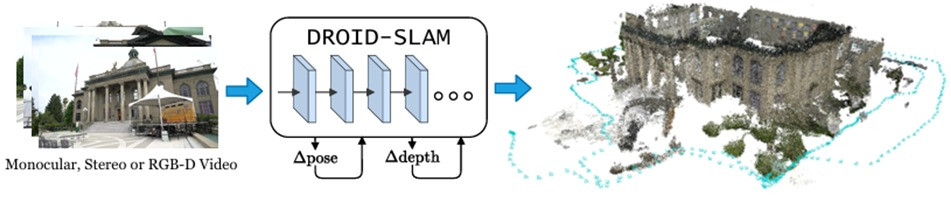
\includegraphics[width=0.8\textwidth]{droid.jpeg}
\caption{DROID-SLAM System Architecture~\cite{teed2021droid}}
\label{fig:droid_slam}
\end{figure}

\subsection{Related Technology 10 -- MAGiC-SLAM Multi-Agent Gaussian Mapping}

MAGiC-SLAM~\cite{yugay2024magic} introduces a multi-agent SLAM framework based on a 3D Gaussian scene representation. Rather than describing the environment as the point clouds or voxels, the model is represented by Gaussian primitives that enable the representation of the scene in an efficient manner, and map merging. The most important contribution of MAGiC-SLAM is that it is capable of fusing maps formed by several robots into a map on a global scale by the means of trajectory alignment and loop closure. This method enhances large indoor en-scalability, vironments and minimizes drift. In a place where numerous delivery robots are used at the same time, e.g. warehouses or hospitals, MAGiC-SLAM provides a viable tool of collaborative mapping and common space understanding.

\begin{figure}[htbp]
\centering
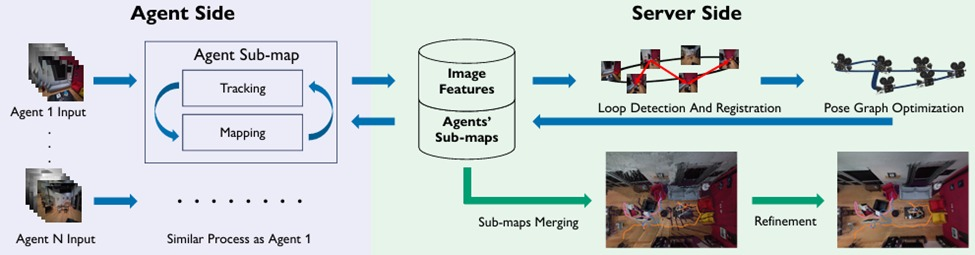
\includegraphics[width=0.8\textwidth]{magic.jpeg}
\caption{Overview of a multi-agent SLAM system~\cite{yugay2024magic}}
\label{fig:magic_slam}
\end{figure}

\subsection{Related Technology 11 -- WildGS-SLAM for Dynamic Environment Mapping}

WildGS-SLAM~\cite{zheng2025wildgs} addresses the challenge of SLAM in dynamic environments using a monocular camera and Gaussian splatting representation. Indoor delivery environments often include moving humans, doors which open and close and moving objects that are capable of corrupting the SLAM map. WildGS-SLAM proposes an uncertain tracking and mapping filter which identifies and eliminates dynamical features in the scene without the use of semantic segmentation or depth sensors. Through uncertainty prediction per-pixel, integrating it with dense bundle adjustment and Gaussian maps optimization, WildGS-SLAM performs a good tracking and high-fidelity mapping in dense indoor environments. This feature is very applicable in the parcel delivery robots which act in real-life enhighly moving and occluding environments.

\begin{figure}[H]
\centering
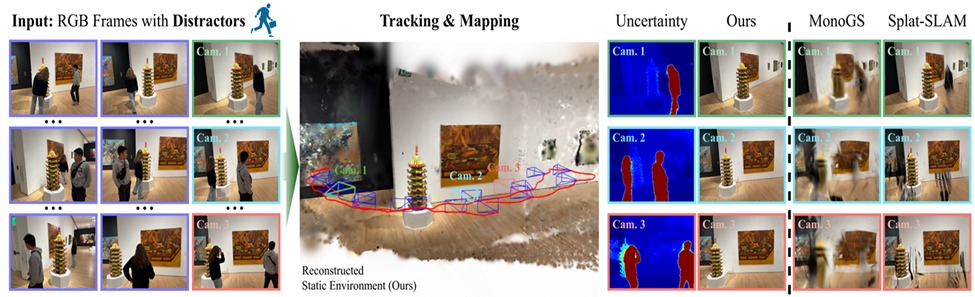
\includegraphics[width=0.8\textwidth]{wild gs.jpeg}
\caption{WildGS-SLAM Overview~\cite{zheng2025wildgs}}
\label{fig:wildgs_slam}
\end{figure}

\begin{table}[htbp]
\centering
\caption{Comparison of SLAM Techniques}
\label{tab:slam_comparison}
\begin{tabular}{|p{3cm}|p{3cm}|p{3cm}|p{3cm}|}
\hline
\textbf{SLAM Method} & \textbf{Strengths} & \textbf{Weaknesses} & \textbf{Application Suitability} \\
\hline
LiDAR-Based SLAM & High mapping accuracy & Expensive hardware & Industrial robotics \\
\hline
Visual SLAM & Cost-effective and flexible & Sensitive to lighting & Indoor mobile robots \\
\hline
DROID-SLAM & High accuracy and robustness & High computational req. & Auto navigation research \\
\hline
MAGiC-SLAM & Supports collaborative mapping & Complex implementation & Multi-robot systems \\
\hline
WildGS-SLAM & Handles moving objects & High processing cost & Dynamic indoor environments \\
\hline
\end{tabular}
\end{table}

Table~\ref{tab:slam_comparison} summarizes different SLAM techniques used for robot localization and mapping. LiDAR-based SLAM provides high accuracy but increases hardware cost. Visual SLAM offers cost-effective mapping using camera data but may be affected by lighting conditions. DROID-SLAM have enhanced accuracy and robustness mapping. Other multi-agent systems such as MAGiC-SLAM are improved collaborative mapping and WildGS-SLAM enhance the performance with respect to dynamic environments. These studies suggest that visual SLAM techniques are based on deep learning enable appropriate performance-cost tradeoff in indoor robotics.

\section{Related Projects}

There are a number of research projects and experimental robotic systems that have made a contribution significantly to the creation of autonomous perception systems, frameworks of navigation and mixed control policies. Such research provides valuable insights for middlewares integration, vision based perception, SLAM advancements, path planning strategies, among others, that impact the design of the proposed autonomous indoor parcel delivery system.

\begin{table}[htbp]
\centering
\caption{Comparative Summary of Related Research Projects in Autonomous Mobile Robot Navigation}
\label{tab:related_projects}
\begin{tabular}{|p{3cm}|p{4.5cm}|p{6cm}|}
\hline
\textbf{Project / Study} & \textbf{Techniques Used} & \textbf{Key Outcomes} \\
\hline
Bonci et al.~\cite{bonci2023ros2} & ROS2 middleware, modular architecture & Demonstrated ROS2 as a scalable platform enabling flexible integration \\
\hline
Gargouri et al.~\cite{gargouri2024cost} & ROS2 Nav2, AMCL, YOLO, fuzzy PID & Developed cost-effective indoor robot with reliable localization \\
\hline
Teed \& Deng~\cite{teed2021droid} & Deep learning visual SLAM, DBA & Provided highly accurate localization and mapping in complex environments \\
\hline
Yugay et al.~\cite{yugay2024magic} & Multi-agent SLAM, distributed mapping & Improved global map consistency and localization accuracy \\
\hline
Zheng et al.~\cite{zheng2025wildgs} & Gaussian splatting SLAM, dynamic filtering & Enhanced SLAM performance in dynamic environments \\
\hline
Cao et al.~\cite{cao2024pure} & Pure pursuit steering, reinforcement learning & Improved trajectory tracking and adaptive velocity control \\
\hline
Song et al.~\cite{song2020smooth} & Bezier curves, PSO optimization & Achieved smoother and kinematically feasible path generation \\
\hline
\end{tabular}
\end{table}

Table~\ref{tab:related_projects} summarizes major research contributions in autonomous mobile robot navigation, highlighting advancements in middleware frameworks, SLAM techniques, perception systems, and path planning methods. The studies reviewed prove the presence of the significance of ROS2 based modular designs, localization and mapping solutions and smarts in navigation. These developments, when added together, provide robust technological basis to develop trustworthy and effective autonomous directly underpin the process taken by the proposed project and are robotic systems.

\section{Related Studies / Research}

We investigated several research studies focusing on different aspects of navigation of autonomous mobile robots which will be useful to design and develop the indoor parcel delivery robot system.

\begin{itemize}
\item \textbf{Hybrid Path Planning Strategies:} In a comparative study, it has been demonstrated that a mixture of classical graph-based algorithms (such as A*) and optimization and learning-based approaches is appropriate.~\cite{ajeil2020grid}.Studies indicate that the hybrid navigation results in improved path optimality, adaptability and computational efficiency.
\item \textbf{Path Smoothing and Trajectory Optimization:}  We found that the raw paths usually contain discontinuities and sharp turns based on the work done on smoothing techniques for the smooth trajectories~\cite{ravankar2018path}. The researches show that the spline based interpolation and curve fitting methods improve the smoothness of the motion, decrease the mechanical stresses and enhance the tracking accuracy.
\item \textbf{PSO-Based Path Optimization:} A large number of studies have been conducted on the field of robot trajectory optimization using Particle Swarm Optimization (PSO)~\cite{song2020smooth}. It has been revealed that PSO can reduce both path length and curvature variation and also reduce energy consumption. The improved PSO variants exhibit faster convergence with better optimization ability.

\item \textbf{Dynamic Obstacle Avoidance in Indoor Environments:} The focus in human-aware navigation research is to incorporate vision sensors into the real-time obstacle avoidance algorithm.The problem of human-aware navigation focuses on the integration of vision-based perception systems with real-time obstacle avoidance algorithms~\cite{kumar2024real}. Research has shown that fusing computer vision models with adaptive motion planning enhances safety and reliability.

\item \textbf{ROS2-Based Autonomous Navigation Frameworks:} There have been a number of studies that have assessed ROS2 middleware for autonomous robotic applications~\cite{hwang2023ros2}. The studies show that ROS2 offers modular architecture, support for real-time communication and enhanced scalability.

\item \textbf{SLAM Performance in Indoor Navigation:} Comparative studies of visual SLAM, LiDAR-based SLAM, and deep learning-based SLAM methods indicate that visual SLAM provides a cost-effective solution for indoor localization~\cite{rosinol2020kimera}.

\item \textbf{Model Predictive Control for Mobile Robots:} MPC has been shown to be effective for handling motion constraints, optimizing the trajectory tracking and enhancing stability in the context of research~\cite{nascimento2023nonlinear}. The controller based on MPC is better than the classical PID controller.

\item \textbf{Simulation-Based Navigation Testing:} The relevance of simulation environments for testing robot navigation algorithms prior to deployment in the real world have been emphasized in the studies~\cite{park2021simulation}. The simulation platforms~\cite{koenig2004gazebo} enable the safe testing of SLAM, obstacle avoidance, and path planning strategies.
\end{itemize}

\section{Limitations and Bottlenecks of the Existing Work}
Although there are some great advancements in the field of autonomous mobile robot locomotion, some of the existing methods are constrained technically and practically and, thus, can only be effective in a real-world delivery scenario. These limitations can be related to difficulties in the optimisation of parameters, the quality of the path-generation, motion control stability, and environmental sensing. The detailed knowledge of these bottlenecks is invaluable to stipulate the areas in which a better navigation strategy and system architecture are justified.
\begin{table}[htbp]
\centering
\caption{Limitations of Existing Work}
\label{tab:limitations}
\begin{tabular}{|p{5cm}|p{9cm}|}
\hline
\textbf{Method / Approach} & \textbf{Limitation} \\
\hline
Default ROS2 Nav2 Framework & Requires extensive parameter tuning and offers limited flexibility for custom strategies \\
\hline
Traditional Path Planning (A*, Dijkstra, RRT) & Often generate jagged paths and show reduced efficiency in dynamic environments \\
\hline
Path Execution Without Smoothing & Produces trajectories that violate kinematic constraints, leading to unstable motion \\
\hline
Fixed-Gain Controllers & Lack adaptability to changing conditions, causing oscillations and poor tracking \\
\hline
Single-Sensor SLAM Methods & May suffer from localization drift or reduced performance in dynamic env. \\
\hline
Limited Dynamic Obstacle Handling & Classical systems often assume static env. and struggle with humans \\
\hline
Lack of Integrated Hybrid Nav Systems & Most studies focus on individual components rather than unified frameworks \\
\hline
\end{tabular}
\end{table}

See Table~\ref{tab:limitations} for the limitations, suggesting a need for more adaptive, integrated, and optimization-driven navigation solutions. To tackle these challenges, advanced perception techniques, smooth and fast route planning, adaptive obstacle management and enhanced adaptive control and dynamic control systems are needed. These observations are one of the most motivating factors that will trigger the development of the proposed autonomous delivery robot system, which aims to overcome these limitations by adopting a hybrid navigation approach and enhancing system integration.

\section{Problem Statement}

Even though the current robotic middleware applications like ROS 2 and the Navigation 2 (Nav2) architecture offer good baseline navigation functions, a number of technical challenges remain. Delivery of parcels manually in large indoor areas is time-consuming, labor intensive and prone to delays. The majority of the current implementations are dependent on pre-configured navigation modules which restricts flexibility of the system. Existing autonomous delivery solutions have severe constraints, including path jagging which breaks the kinematic limit of differentially-driven robots. The additional effects of path smoothing and trajectory optimization are unstable in robot motion. Moreover, a lot of implementations cannot deal with dynamic obstacle avoidance. Localization accuracy is also a major problem, especially when it comes to visual static or dynamic environments. More so, traditional methods of motion control like fixed-gain controllers demand a lot of parameter adjustment. To address these challenges, this project will provide an integrated solution with ROS 2 middleware-based robot that encompasses effective SLAM-based localization and hybrid path planning.

\section{Summary}

In this chapter, literature review was discussed including the principles of autonomous mobile robots navigation such as robotic perception, localization (SLAM) and path planning, trajectory smoothing and motion control strategies have been discussed. It also examined ROS 2 middlewares and simulation tools helpful in autonomous robot operation. The comparison of similar projects and research works provided information about the necessity of combining localization, planning, control, and perception modules. The shortcomings of the current navigation methods underscore the necessity to establish incorporated and more tailored navigation systems. Hence, the proposed project will be aimed at the deploying of a ROS 2-based autonomous parcel delivery robot as a solution to the existing gap between the theoretical concepts of navigation and the real-world application of robots.